%%%%%%%%%%%%%%%%%%%%%%%%%%%
% IEEE Submission Dashboard - https://ieee.atyponrex.com/submission/dashboard
%%%%%%%%%%%%%%%%%%%%%%%%%%%

% IEEE Transactions on human--machine systems
% https://ieeexplore.ieee.org/xpl/mostRecentIssue.jsp?punumber=6221037

%---------------------------------------------------------------------
% \documentclass[10pt,journal,compsoc]{IEEEtran}
% \documentclass[lettersize,journal]{IEEEtran}
% \documentclass[letterpaper,journal]{IEEEtran}
\documentclass[journal]{IEEEtran}
% ==== Core packages (normalized) ====

% How to hide statements:
%   - To enable  tags: \iftrue  and \fi
%   - To disable tags: \iffalse and \fi
% How to turn-on (or turn-off) page number:
%   - To turn-on  the page number: {plain}
%   - To turn-off the page number: {empty}
% Usage (Syntax):
%   \documentstyle[twocolumn]{article}
%   \pagestyle{empty}
%    ...
%   \maketitle
%   \thispagestyle{empty}

% How to print the page number at each page
\pagestyle{empty}

\usepackage[T1]{fontenc}
\usepackage[utf8]{inputenc}
\usepackage{microtype}
\usepackage{amsmath,amssymb}
\usepackage{amsthm}  % theorem 환경을 사용하기 위한 필수 패키지
%\usepackage{amsmath}
%\usepackage{amssymb}
\usepackage{makecell}
%\usepackage{amsmath,amsfonts,amssymb,mathtools}
%\usepackage{amsthm}
\usepackage{graphicx}
\usepackage{booktabs}
\usepackage{siunitx}
\usepackage{xspace}
\usepackage{pifont}
% Checkmark / Xmark symbols
\newcommand{\cmark}{\ding{51}}
\newcommand{\xmark}{\ding{55}}

\usepackage{listings}
\usepackage{xcolor}
\usepackage{xurl}
\usepackage{url}

% Hyperlinks to content
% \usepackage[linktocpage=true]{hyperref}
% \usepackage{hyperref}
% \usepackage[nameinlink]{cleveref}
% \usepackage[hidelinks]{hyperref}
\usepackage[colorlinks=true,linkcolor=blue,citecolor=blue,urlcolor=black]{hyperref}

\usepackage{cleveref}
%\usepackage{amsmath,amsfonts}
% \usepackage{algorithmic}
\usepackage{algorithm}
\usepackage{array}
\usepackage[caption=false,font=normalsize,labelfont=sf,textfont=sf]{subfig}
\usepackage{textcomp}
\usepackage{stfloats}
\usepackage{verbatim}
\usepackage{cite}
%\hyphenation{op-tical net-works semi-conduc-tor IEEE-Xplore}
%\usepackage{amssymb,amsmath,amsthm,mathtools}
%\usepackage{hyphenat}

%% ------------- ORC ID Template: Start ----------------------
% https://tex.stackexchange.com/questions/498688/orcid-in-latex-file-of-ieee-trans-in-a-customized-position

\usepackage{scalerel}
\usepackage{tikz}
\usetikzlibrary{svg.path,positioning,arrows.meta,shapes.geometric,calc}

\definecolor{orcidlogocol}{HTML}{A6CE39}
\tikzset{
orcidlogo/.pic={
\fill[orcidlogocol] svg{M256,128c0,70.7-57.3,128-128,128C57.3,256,0,198.7,0,128C0,57.3,57.3,0,128,0C198.7,0,256,57.3,256,128z};
\fill[white] svg{M86.3,186.2H70.9V79.1h15.4v48.4V186.2z}
svg{M108.9,79.1h41.6c39.6,0,57,28.3,57,53.6c0,27.5-21.5,53.6-56.8,53.6h-41.8V79.1z M124.3,172.4h24.5c34.9,0,42.9-26.5,42.9-39.7c0-21.5-13.7-39.7-43.7-39.7h-23.7V172.4z}
svg{M88.7,56.8c0,5.5-4.5,10.1-10.1,10.1c-5.6,0-10.1-4.6-10.1-10.1c0-5.6,4.5-10.1,10.1-10.1C84.2,46.7,88.7,51.3,88.7,56.8z};
}
}

\newcommand\orcidicon[1]{\href{https://orcid.org/#1}{\mbox{\scalerel*{

\begin{tikzpicture}[yscale=-1,transform shape]
    \pic{orcidlogo};
\end{tikzpicture}
}{|}}}}

%% ------------- ORC ID Template: End ----------------------

\providecommand{\cmark}{\ding{51}}
\providecommand{\xmark}{\ding{55}}
\providecommand{\etal}{\textit{et al.}\xspace}
\DeclareMathOperator{\E}{\mathbb{E}}
\DeclareMathOperator{\Var}{\mathrm{Var}}

\theoremstyle{plain}
\newtheorem{theorem}{Theorem}[section]
\newtheorem{lemma}{Lemma}[section]
\newtheorem{corollary}{Corollary}[section]
\lstdefinelanguage{json}{
basicstyle=\ttfamily\small,
numbers=left,
numberstyle=\tiny,
stepnumber=1,
showstringspaces=false,
breaklines=true
}
\lstset{frame=single}
% === End patch ===

\IEEEoverridecommandlockouts

%####################################################### Geunsik Area ###########

\usepackage{algorithm}
\usepackage{algpseudocode}

% LaTeX에서 유니코드(①, ② 등)를 직접 사용
\usepackage{pifont}

% theorem, algorithm 가독성위해 디자인 개선
\usepackage[most]{tcolorbox}
\tcbuselibrary{listings}

%% To keep strictly tuned whitespace rules among sections (e.g., section, subsection, and subsubsection)
%% for decreasing or increasing the vertical space between sections
\usepackage{titlesec}
\titlespacing*{\section}{0.70pt}{0.50\baselineskip}{0.20\baselineskip}
\titlespacing*{\subsection}{0.70pt}{0.50\baselineskip}{0.20\baselineskip}
\titlespacing*{\subsubsection}{0.70pt}{0.50\baselineskip}{0.20\baselineskip}

%% Reduce vertical space (padding) after figure (a big effect)
%% Warning: "Text page 7 contains only floats."
%% https://www.reddit.com/r/LaTeX/comments/b4mipa/how_to_decrease_space_between_paragraph_and/
\setlength{\textfloatsep}{0.70pt}
\setlength{\abovecaptionskip}{0.70pt}
\setlength{\belowcaptionskip}{0.70pt}

\theoremstyle{definition}
\newtheorem{definition}{Definition}[section]
\urlstyle{tt}

\newcommand{\Lninetyfive}{L_{95}}
\newcommand{\Jain}{\mathcal{J}}
\providecommand{\cmark}{\ding{51}}
\providecommand{\xmark}{\ding{55}}

% JSON language for listings
\lstdefinelanguage{json}{
basicstyle=\ttfamily\small,
numbers=left, numberstyle=\tiny, stepnumber=1,
showstringspaces=false,
breaklines=true
}

% Listings setup (handles code blocks and JSON/diff-like listings)
\lstset{basicstyle=\ttfamily\small, breaklines=true, columns=fullflexible, showstringspaces=false}

% Minimal JSON language for listings
\lstdefinelanguage{json}{
basicstyle=\ttfamily\small,
showstringspaces=false,
morestring=[b]",
morecomment=[l]{//},
literate=
*{0}{{{\color{black}0}}}{1}
{1}{{{\color{black}1}}}{1}
{2}{{{\color{black}2}}}{1}
{3}{{{\color{black}3}}}{1}
{4}{{{\color{black}4}}}{1}
{5}{{{\color{black}5}}}{1}
{6}{{{\color{black}6}}}{1}
{7}{{{\color{black}7}}}{1}
{8}{{{\color{black}8}}}{1}
{9}{{{\color{black}9}}}{1}
{:}{{{\color{black}{:}}}}{1}
{,}{{{\color{black}{,}}}}{1}
{"}{{{\color{black}{"}}}}{1}
}


\begin{document}

    %----------------------------------------\input{./001-title}

    \title{From Alerts to Actions: A Human--AI Decision System for Reliable Action Execution Under Disaster Risk}

    %---------------------------------- \input{./003-author}

    \author{

    % for ORC-ID
    \IEEEauthorblockN{
    Geunsik Lim$^{\textsuperscript{\orcidicon{0000-0003-1845-7132}}}$
    }


    \thanks{G. Lim is with the Department of Electrical and Computer Engineering, Sungkyunkwan University, 2066, Seobu-ro, Jangan-gu, Suwon 16419, South Korea (e-mail: leemgs@g.skku.edu). }

    }

    % The paper headers
    % \markboth{Journal of \LaTeX\ Class Files,~Vol.~14, No.~8, August~2015}%
    % {Shell \MakeLowercase{\textit{et al.}}: Bare Demo of IEEEtran.cls for IEEE Transactions on Magnetics Journals}

    \markboth{IEEE Transactions on Human-Machine Systems}{Lim: From Alerts to Actions: A Human--AI Decision System Under Disaster Risk}

    % make the title area
    \maketitle

    \thispagestyle{empty}%

    % -----------------------------\input{./005-abstract}
    \begin{abstract}
        Human--AI decision systems are increasingly used in situations where an inappropriate or delayed human action can have serious consequences. Improvements in the predictive accuracy of AI do not, by themselves, translate into appropriate human action. Drawing on the joint cognitive systems perspective, which evaluates the human and the machine as a single system, we present the \emph{Action-Centered Human--AI Decision Framework (ACHDF)}. ACHDF instantiates uncertainty-aware risk estimation, guardrailed AI recommendations, and human-in-the-loop escalation for disaster-response decision support, and it treats human action execution as the primary evaluation outcome. In a counterbalanced within-subjects study ($n=52$), we compared an ACHDF-based prototype with a conventional dashboard in a simulated disaster-response decision task. Compared with the dashboard, the ACHDF condition was associated with a higher action execution rate, shorter response latency, lower self-reported workload (NASA--TLX), and higher perceived trust and usability. Because the two conditions differed in several features at once, the results describe the effect of the integrated ACHDF configuration rather than of individual components. We discuss implications for the design of human--AI decision support under uncertainty. Validation in other domains and with professional operators remains future work.
    \end{abstract}

    \begin{IEEEkeywords}
        Human--AI decision systems, joint cognitive systems, adaptive automation, human-in-the-loop, trust in automation, cognitive workload, action execution
    \end{IEEEkeywords}

    %--------------------------------------- \input{./010-introduction}
\section{Introduction}
\IEEEPARstart{H}{uman}--AI decision systems are increasingly used in situations with high uncertainty, high stakes, and severe time pressure \cite{Bach2024Access,PerezCerrolaza2024CSUR,Yang2022THMSReview}. Examples include healthcare triage, supervision of autonomous vehicles, industrial safety, and emergency response \cite{Birkmann2013NatHazards,Sandoval2023IJDRS,Rokhideh2025IJDRS,Rao2024IJDRS,Charan2024,lim2026generativeaidrivenreliabilitylayer}. In these settings, AI is mainly used to improve prediction. Human--machine systems research, however, has repeatedly shown that better predictions do not necessarily lead to appropriate human action \cite{Lai2023FAccT,Muller2022CHIWORK,Hodgson2013THMS}. In disaster response, effective action also depends on community-level coordination, resilient communications, and distributed sensing and reporting \cite{Stephens2022SIGDOC,Longo2025PMC,Yang2005MobiHoc}.

When information is incomplete or uncertain, operators must weigh risk, confidence, and responsibility while working with machines \cite{Yang2022THMSReview,Bach2024Access}. AI systems, however, often communicate their uncertainty poorly or only implicitly \cite{McAllister2017IJCAI,Weidinger2022FAccT,Miller2019XRDS}. Their outputs are typically shown as probabilities or alarms, with little support for turning them into action \cite{Miller2019XRDS,Bach2024Access}. The human is left to close the loop between prediction and action, often under cognitive stress \cite{Hodgson2013THMS,Zhang2022THMS}.

Although machine learning has greatly improved predictive accuracy \cite{Mai2024TOS,PerezCerrolaza2024CSUR}, accuracy does not necessarily translate into human performance \cite{Lai2023FAccT,Yang2022THMSReview}. Operators may wait for confirmation before acting, disregard advice they do not trust, or over-rely on an AI whose accuracy is overstated \cite{Hodgson2013THMS,Raji2019AIES,Raji2022CACM,Parasuraman2010}. Human action therefore depends not only on what the system predicts, but also on how the prediction is communicated and how control is shared with the user. Without explicit support for appropriate trust, workload management, and human override, decision support can increase automation bias or workload and lose its intended benefit \cite{Hodgson2013THMS,Zhang2022THMS,Bach2024Access,Lee2004}.

These concerns are not new to cognitive systems engineering. The joint cognitive systems (JCS) perspective holds that a human and a machine working together form a single cognitive system, and that this system should be evaluated by the outcomes it jointly produces, not by the performance of the machine alone \cite{Hollnagel2005JCS,Woods2006JCS}. Research on adaptive automation and levels of automation has likewise studied how support should change with task demands while keeping the human in control \cite{Parasuraman2000LOA,Kaber2004,Scerbo2007}. Much current work on AI-based decision support, however, still evaluates systems by prediction accuracy or usability rather than by whether the human--AI system produces appropriate and timely action \cite{Lai2023FAccT,Muller2022CHIWORK,Yang2022THMSReview,lim2026generativeaidrivenreliabilitylayer}. This paper applies the JCS perspective to AI-assisted disaster-response decision support and tests it empirically.

We address the following, deliberately scoped research question:
\begin{quote}
    \emph{Compared with a conventional dashboard, is an ACHDF-based decision support system associated with better action execution in a simulated, high-uncertainty disaster-response task, and how does it relate to response latency, workload, and trust?}
\end{quote}
We specified the following hypotheses before data collection:
\begin{itemize}
    \item \textbf{H1 (primary):} The Action Execution Rate (AER) is higher in the AI-assisted (ACHDF) condition than in the baseline condition.
    \item \textbf{H2 (secondary):} Response latency is shorter in the AI-assisted condition.
    \item \textbf{H3 (secondary):} Self-reported workload (NASA--TLX) is lower in the AI-assisted condition.
    \item \textbf{H4 (secondary):} Perceived trust and usability are higher in the AI-assisted condition.
\end{itemize}
In this study, action execution is the primary outcome. Response latency, workload, trust, and usability are secondary outcomes. Trust and workload also act as \emph{design considerations} that shaped how information is presented, but the implemented system does not measure or adapt to them at run time (Section~\ref{sec:constructs}).

The contributions of this paper are as follows. First, we apply the JCS principle of evaluating joint human--machine outcomes to AI-assisted disaster decision support, with action execution as the primary evaluation outcome. The principle itself is established in cognitive systems engineering \cite{Hollnagel2005JCS,Woods2006JCS}. Our contribution is to make it concrete for an application area where AI systems are usually evaluated by accuracy alone. Second, we present ACHDF, a domain-specific instantiation of the JCS and adaptive function allocation perspectives that combines uncertainty-aware risk estimation, guardrailed AI recommendations, and uncertainty- and criticality-triggered escalation, while the human keeps final decision authority. Third, we report a controlled within-subjects evaluation ($n=52$) that compares the integrated ACHDF configuration with a conventional dashboard on action execution, response latency, workload, trust, and usability. Because several features differed between conditions, this evaluation does not isolate the contribution of individual ACHDF components.


    %----------------------------- \input{./020-related_work}
\section{Related Work}
This section reviews four research streams that ACHDF builds on: joint cognitive systems and adaptive function allocation, which form the conceptual basis of the framework; human--machine decision support; trust, workload, and automation bias; and AI assistance in high-stakes environments. It closes with a short note on the information sources that feed disaster decision support.

\subsection{Joint Cognitive Systems and Adaptive Function Allocation}
Cognitive systems engineering treats a human operator and the technology the operator works with as a \emph{joint cognitive system} (JCS). The unit of analysis is the joint system and the outcomes it produces in its work environment, not the machine's internal performance \cite{Hollnagel2005JCS,Woods2006JCS}. From this perspective, evaluating decision support by the actions the joint system executes is a natural consequence of the design stance, not a new concept. ACHDF adopts this stance explicitly.

A second relevant body of work addresses how functions should be allocated between humans and automation. Parasuraman \emph{et al.} distinguish types of automation (information acquisition, information analysis, decision selection, and action implementation) and levels of automation within each type \cite{Parasuraman2000LOA}. Adaptive automation changes the level or type of support in response to task demands, operator state, or critical events \cite{Scerbo2007,Kaber2004}. Empirical studies show that intermediate levels of decision support can improve performance, but that higher levels can reduce situation awareness and leave operators poorly prepared to intervene when automation fails \cite{Kaber2004,Parasuraman2010}.

ACHDF relates to this literature in three ways. (i) In the terms of Parasuraman \emph{et al.} \cite{Parasuraman2000LOA}, it automates information analysis and decision selection (risk estimation and recommendation), but it never automates action implementation: the human always executes the action. (ii) Its adaptation is \emph{event-triggered}. The form of support changes when estimated uncertainty, action criticality, or a policy check crosses a threshold (Algorithm~\ref{alg:escalation}), not in response to measured operator workload or physiological state. (iii) What changes is the \emph{level and form of AI support}, from a bounded recommendation to an escalated presentation of evidence and options. Decision authority does not move between the AI and the human. ACHDF therefore does not propose a new allocation theory. It is a domain-specific instantiation of these principles for AI-generated recommendations in disaster response.

\subsection{Human--Machine Decision Support Systems}
Human--machine decision support has been studied extensively in supervisory control, command and control, and complex socio-technical systems \cite{Hodgson2013THMS,Yang2022THMSReview,Bach2024Access}. Early work focused on how automation can make information processing faster and more consistent, and on the risks of misallocating functions between humans and automation \cite{Hodgson2013THMS,Zhang2022THMS}.
More recent work shows that what matters is not only the quality of the information provided, but also how recommendations enter the human decision process \cite{Lai2023FAccT,Muller2022CHIWORK}. Systems that only display information or predictions leave interpretation and decision making to the user, which is especially costly under time pressure \cite{Bach2024Access,PerezCerrolaza2024CSUR}. This has motivated decision support that provides actionable recommendations while keeping the human in control and responsible \cite{Assaad2023TAS,Yang2022THMSReview}.

\subsection{Trust, Workload, and Automation Bias}
Trust and cognitive workload are important constructs used to explain the performance of human--machine systems \cite{Hodgson2013THMS,Bach2024Access}. Trust in automation is commonly defined as the attitude that an agent will help achieve an individual's goals in a situation characterized by uncertainty and vulnerability. \emph{Appropriate} (calibrated) trust means that reliance matches the actual capabilities of the automation \cite{Lee2004}. Over-trust can lead to misuse and automation bias, in which errors made by the automation go undetected. Under-trust leads to disuse of useful support \cite{Lee2004,Parasuraman2010,Raji2019AIES,Raji2022CACM}.

Automation bias and complacency are most likely when automation is highly but not perfectly reliable and when its uncertainty is not represented \cite{Parasuraman2010,Weidinger2022FAccT}. Representing uncertainty and giving humans the opportunity to verify decisions has been proposed as a way to support appropriate reliance \cite{Miller2019XRDS,Bach2024Access}. Assessing calibration directly requires comparing reliance with the correctness of the automation's advice, including trials in which the advice is wrong \cite{Lee2004,Parasuraman2010}. Workload is commonly measured with the NASA Task Load Index (NASA--TLX) \cite{Hart1988} and has been examined as a factor in the relationship between automation and performance \cite{Hodgson2013THMS,Yang2022THMSReview}. Decision support that reduces information integration and action selection demands is expected to reduce workload and response time \cite{Lai2023FAccT,Muller2022CHIWORK}.

\subsection{AI Assistance in High-Stakes Environments}
AI-assisted decision systems are increasingly used for time-critical decisions in healthcare, aviation, and emergency management \cite{PerezCerrolaza2024CSUR,Bach2024Access,Rokhideh2025IJDRS,Rao2024IJDRS}. Empirical studies show that higher predictive accuracy in these settings does not guarantee better human performance \cite{Lai2023FAccT,Yang2022THMSReview}.

Work on responsible and explainable AI stresses human-in-the-loop controls and governance, particularly in safety-critical applications \cite{Weidinger2022FAccT,Assaad2023TAS,Miller2019XRDS,PerezCerrolaza2024CSUR}. Most of this work, however, is conceptual or algorithm-centric and does not measure human behavior. Few studies have examined empirically how specific design features, such as uncertainty-aware escalation and guardrails, affect the actions humans take \cite{Bach2024Access,Lai2023FAccT}.

\subsection{Information Sources for Disaster Decision Support}
In disaster response, the input to the risk-modeling layer of ACHDF (Section~\ref{sec:system}) comes from heterogeneous sensor networks, ad hoc communications, and community reporting, whose robustness affects the quality of the signal available for decision making \cite{Yang2005MobiHoc,Longo2025PMC,Stephens2022SIGDOC}. Network-analytic methods such as community detection have been used to structure such large and noisy information environments \cite{Wakita2007WWW,Prokhorenkova2019WWW,Xian2025WWW,Slota2019SC,Sun2014FSKD,Rezaei2015ASONAM,Akhter2022ICCA,Sun2011InformationSciences,Havens2013TFUZZ,Vehlow2013TVCG,Zhang2012KDD,Cao2020ICIIP,Li2022AppliedIntelligence,Duan2014KDD}. These upstream methods are outside the scope of this paper. They are mentioned only because the uncertainty that ACHDF must represent originates in them.


%-----------------------------input{./050-design}

    \begin{figure}[t]
        \centering
        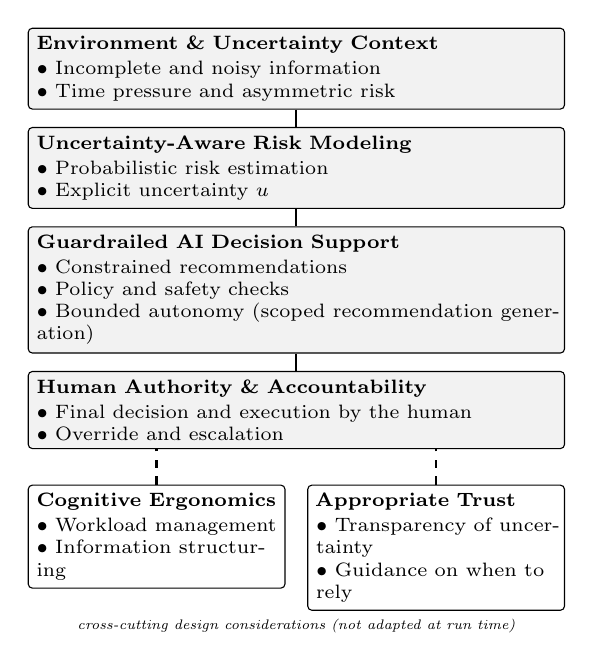
\begin{tikzpicture}[
            font=\scriptsize, node distance=2.2mm,
            layer/.style={draw, rounded corners=1.5pt, fill=gray!10, text width=6.6cm, align=left, inner sep=3pt},
            cross/.style={draw, rounded corners=1.5pt, fill=white, text width=3.05cm, align=left, inner sep=3pt, minimum height=1.25cm, anchor=north},
            ln/.style={thick}]
            \node[layer] (l1) {\textbf{Environment \& Uncertainty Context}\\[1pt]
                $\bullet$ Incomplete and noisy information\\ $\bullet$ Time pressure and asymmetric risk};
            \node[layer, below=of l1] (l2) {\textbf{Uncertainty-Aware Risk Modeling}\\[1pt]
                $\bullet$ Probabilistic risk estimation\\ $\bullet$ Explicit uncertainty $u$};
            \node[layer, below=of l2] (l3) {\textbf{Guardrailed AI Decision Support}\\[1pt]
                $\bullet$ Constrained recommendations\\ $\bullet$ Policy and safety checks\\
                $\bullet$ Bounded autonomy (scoped recommendation generation)};
            \node[layer, below=of l3] (l4) {\textbf{Human Authority \& Accountability}\\[1pt]
                $\bullet$ Final decision and execution by the human\\ $\bullet$ Override and escalation};
            \draw[ln] (l1) -- (l2); \draw[ln] (l2) -- (l3); \draw[ln] (l3) -- (l4);
            \node[cross, anchor=north west] (ce) at ($(l4.south west)+(0,-0.45)$) {\textbf{Cognitive Ergonomics}\\[1pt]
                $\bullet$ Workload management\\ $\bullet$ Information structuring};
            \node[cross, anchor=north east] (at) at ($(l4.south east)+(0,-0.45)$) {\textbf{Appropriate Trust}\\[1pt]
                $\bullet$ Transparency of uncertainty\\ $\bullet$ Guidance on when to rely};
            \draw[ln, dashed] (ce.north) -- (ce.north |- l4.south);
            \draw[ln, dashed] (at.north) -- (at.north |- l4.south);
            \node[font=\tiny\itshape, anchor=north] at ($(ce.south)!0.5!(at.south)+(0,-0.12)$) {cross-cutting design considerations (not adapted at run time)};
        \end{tikzpicture}
        \caption{Conceptual design layers of the Action-Centered Human--AI Decision Framework (ACHDF).
The framework structures human--AI decision support into four layered components: environment and uncertainty context, uncertainty-aware risk modeling, guardrailed AI decision support, and preserved human authority and accountability. Appropriate trust \cite{Lee2004} and cognitive ergonomics are cross-cutting design considerations that guided interface design. Trust and workload are also measured as evaluation outcomes. They are not adapted at run time (Table~\ref{tab:constructs}).}
        \label{fig:achdf_concept}
    \end{figure}

    \begin{figure}[t]
        \centering
        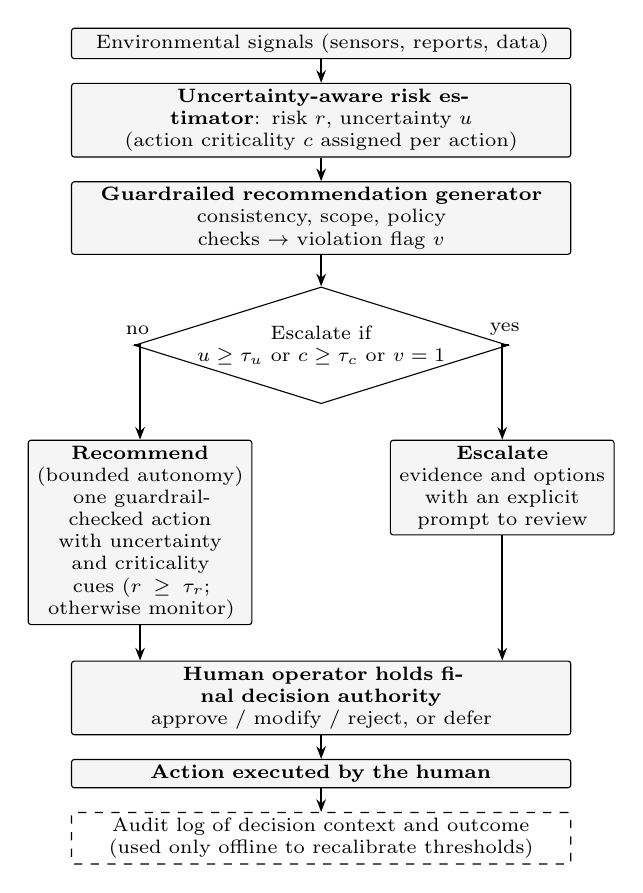
\begin{tikzpicture}[
            font=\scriptsize, node distance=3mm,
            box/.style={draw, rounded corners=1pt, align=center, fill=gray!8, text width=#1, inner sep=2pt},
            box/.default=6.2cm,
            dec/.style={draw, diamond, aspect=3.2, align=center, fill=white, inner sep=0pt},
            arr/.style={-{Stealth[length=1.6mm]}, thick}]
            \node[box] (env) {Environmental signals (sensors, reports, data)};
            \node[box, below=of env] (risk) {\textbf{Uncertainty-aware risk estimator}: risk $r$, uncertainty $u$\\(action criticality $c$ assigned per action)};
            \node[box, below=of risk] (gen) {\textbf{Guardrailed recommendation generator}\\consistency, scope, policy checks $\rightarrow$ violation flag $v$};
            \node[dec, below=4mm of gen] (pol) {Escalate if\\$u \ge \tau_u$ or $c \ge \tau_c$ or $v = 1$};
            \node[box=2.7cm, anchor=north] (rec) at ($(pol.south)+(-2.3,-0.45)$) {\textbf{Recommend} (bounded autonomy)\\one guardrail-checked action with uncertainty and criticality cues ($r \ge \tau_r$; otherwise monitor)};
            \node[box=2.7cm, anchor=north] (esc) at ($(pol.south)+(2.3,-0.45)$) {\textbf{Escalate}\\evidence and options with an explicit prompt to review};
            \node[box, anchor=north] (hum) at ($(rec.south -| pol.south)+(0,-0.45)$) {\textbf{Human operator holds final decision authority}\\approve / modify / reject, or defer};
            \node[box, below=of hum] (act) {\textbf{Action executed by the human}};
            \node[box, below=of act, fill=white, dashed] (log) {Audit log of decision context and outcome\\(used only offline to recalibrate thresholds)};
            \draw[arr] (env) -- (risk); \draw[arr] (risk) -- (gen); \draw[arr] (gen) -- (pol);
            \draw[arr] (pol.west) -| node[above, pos=0.3] {no} (rec.north);
            \draw[arr] (pol.east) -| node[above, pos=0.3] {yes} (esc.north);
            \draw[arr] (rec.south) -- (rec.south |- hum.north);
            \draw[arr] (esc.south) -- (esc.south |- hum.north);
            \draw[arr] (hum) -- (act); \draw[arr] (act) -- (log);
        \end{tikzpicture}
        \caption{Operational workflow of the proposed human--AI decision system.
The escalation test follows Algorithm~\ref{alg:escalation}. Depending on the estimated uncertainty, the action criticality, and the guardrail policy checks, the system either presents a bounded recommendation or escalates the case for human review with evidence and options (when $r < \tau_r$ and no trigger fires, the system only monitors). In both modes, the human operator holds final decision and execution authority. Trust and workload are not adapted at run time. The audit log is used only offline.}
        \label{fig:system_overview}
    \end{figure}

    \section{System Overview and Architecture}
    \label{sec:system}
    This section introduces the proposed human--AI decision system and its architectural elements. The system is non-autonomous and human-centric: the AI analyzes information and proposes options, and the human decides and acts. The architecture follows the \textbf{Action-Centered Human--AI Decision Framework (ACHDF)}, which, following the joint cognitive systems perspective \cite{Hollnagel2005JCS,Woods2006JCS}, treats the human operator and the AI as one decision system and takes appropriate human action as the system's goal.

    A conceptual overview of the proposed action-centered architecture is illustrated in Fig.~\ref{fig:achdf_concept}.
As shown in the figure, ACHDF is organized into four primary design layers. The \emph{environment and uncertainty context} layer captures incomplete, time-pressured, and asymmetric risk conditions that characterize high-stakes decision ecologies. Built on top of this, the \emph{uncertainty-aware risk modeling} layer produces probabilistic risk estimates together with explicit confidence and uncertainty bounds. These estimates are then translated into constrained, policy-aligned options within the \emph{guardrailed AI decision support} layer, which ensures that generated recommendations remain consistent with operational and safety constraints. Finally, the \emph{human authority and accountability} layer preserves human control through oversight, override, and responsibility mechanisms. The two cross-cutting elements at the bottom of the figure, appropriate trust and cognitive ergonomics, are design considerations. They determined which cues are shown (e.g., explicit uncertainty indicators) and how much information is shown at once. The implemented system does not measure them or adapt to them at run time.

The run-time behavior of these layers is depicted in Fig.~\ref{fig:system_overview}.
When model uncertainty is low and the action is not critical, the system presents a tightly scoped, action-oriented recommendation. We call this mode \emph{bounded autonomy}. The term refers only to the AI's freedom in \emph{generating} a recommendation, which is bounded by guardrails. It does not mean that the AI executes actions or holds decision authority. When uncertainty, criticality, or a policy check exceeds its threshold, the system switches to \emph{escalation}: instead of a single recommendation, it presents the evidence and the available options and explicitly asks the operator to review them, and the operator can approve, modify, or reject the suggested action. Thus, what varies between the two modes is the \emph{level and form of AI support}. Final decision and execution authority stays with the human in both modes. Operator responses and outcomes are logged for audit and for offline recalibration of the thresholds.

    \subsection{Constructs and Their Roles}
    \label{sec:constructs}
    Table~\ref{tab:constructs} summarizes the role of each ACHDF construct, i.e., whether it is a design input, a system state, a design consideration, or an evaluation outcome, together with its operational definition in the implemented system.

\begin{table*}[t]
\centering
\caption{ACHDF Constructs: Role, Operational Definition, and Implementation}
\label{tab:constructs}
\begin{tabular}{p{2.4cm} p{3.4cm} p{10.6cm}}
\toprule
\textbf{Construct} & \textbf{Role in ACHDF} & \textbf{Operational definition / implementation} \\
\midrule
Uncertainty $u$ & Design input; determines system mode & Dispersion of the posterior risk estimate (Section~\ref{sec:risk}); compared with threshold $\tau_u$. \\
Criticality $c$ & Design input; determines system mode & Severity of the consequences if the recommended action is wrong or delayed (cost of error); compared with threshold $\tau_c$. \\
Guardrails & Constraint on recommendation generation & Rule-based checks applied to every generated recommendation (Section~\ref{sec:guardrails}). A recommendation that fails a check is withheld and the case is escalated ($v=1$ in Algorithm~\ref{alg:escalation}). \\
Bounded autonomy & System mode (``recommend'') & The AI presents one scoped, guardrail-checked recommendation. The AI never executes actions; the human decides and acts. \\
Escalation & System mode (``escalate'') & Triggered if $u \ge \tau_u$, $c \ge \tau_c$, or a policy check fails ($v=1$). The system presents evidence and options and asks the operator to approve, modify, or reject. \\
Trust & Design consideration; secondary outcome & Shaped interface design (explicit uncertainty and criticality cues). Measured post-condition by questionnaire (Section~\ref{sec:measures}). Not adapted at run time. \\
Workload & Design consideration; secondary outcome & Shaped interface design (single consolidated view, action-oriented phrasing). Measured post-condition by NASA--TLX \cite{Hart1988}. Not adapted at run time. \\
Action execution & Primary outcome & Measured by AER (Section~\ref{sec:measures}). \\
\bottomrule
\end{tabular}
\end{table*}

    \subsection{Design Goals and Human-in-the-Loop Principles}
    The design of the proposed system is informed by three key goals that are derived from the fundamental principles of ACHDF.

    \textbf{Goal 1 --- Enabling Human Action Execution.}
    The system should support \emph{human action execution} effectively, as opposed to only improving situational awareness and prediction accuracy.

    \textbf{Goal 2 --- Supporting Appropriate Trust.}
    The system should support appropriate trust \cite{Lee2004} by making its uncertainty, model limitations, and potential failure modes explicit, so that users can judge when to rely on its outputs and when to rely on their own judgment.

    \textbf{Goal 3 --- Preserving Human Authority.}
    The system should preserve human authority in high-risk decisions. Human operators always hold the final decision-making and execution authority.

    To meet these goals, the AI provides decision scaffolding and action-oriented recommendations, and the human remains responsible for executing actions. In the terms of Parasuraman \emph{et al.} \cite{Parasuraman2000LOA}, the system automates information analysis and decision selection, but not action implementation. The level and form of support are adapted to the estimated uncertainty and the criticality of the action (uncertainty-governed adaptation of support).

    \subsection{Probabilistic Risk Estimation With Uncertainty}
    \label{sec:risk}
    The risk estimation module provides risk assessments together with uncertainty representations. Rather than a point estimate, the module outputs a posterior risk distribution, from which the risk level $r$ and the uncertainty $u$ are derived.
    This paper focuses on how the risk estimate and its uncertainty are used in the human--AI interaction, not on the risk model itself. The model's estimation procedure and calibration are therefore not evaluated here (Section~\ref{sec:lim_reporting}).

    \textbf{Role in ACHDF.}
    The risk level is interpreted together with its uncertainty to decide whether the system presents a bounded recommendation or escalates (Algorithm~\ref{alg:escalation}). Explicitly representing uncertainty is intended to avoid conveying false precision.

    \subsection{Guardrailed AI Recommendation Module}
    \label{sec:guardrails}
    A generative AI module converts the risk estimate into a recommended action and a short justification.

    \textbf{Role in ACHDF.}
    Every generated recommendation passes through guardrails before it is shown: (i) a \emph{consistency check} ensures that the recommended action does not contradict the risk estimate (e.g., no ``no action needed'' message when $r \ge \tau_r$); (ii) a \emph{scope check} ensures that the recommendation is selected from the set of permitted actions for the scenario; and (iii) a \emph{policy check} ensures compliance with operational and safety rules. A recommendation that fails any check is not shown; instead, the case is escalated ($v=1$).
    The specific rule sets, the generative model configuration, and the scale and thresholds for criticality are not reported in this paper (Section~\ref{sec:lim_reporting}).
    Each recommendation is displayed with its criticality and confidence cues. By bounding the generative output within a structured decision process, the module aims to keep AI support assistive rather than prescriptive and to limit hallucination and overgeneralization.
    \begin{algorithm}[t]
        \caption{Uncertainty-aware escalation and human override policy}
        \label{alg:escalation}
        \begin{algorithmic}[1]
            \Require risk estimate $r$, uncertainty $u$, action criticality $c$
            \Require policy-violation flag $v \in \{0,1\}$ from guardrail checks
            \Require thresholds $\tau_r, \tau_u, \tau_c$
            \State $\textsc{mode} \leftarrow \text{``assist''}$
            \If{$u \ge \tau_u$ \textbf{or} $c \ge \tau_c$ \textbf{or} $v = 1$}
            \State $\textsc{mode} \leftarrow \text{``escalate''}$ \Comment{route to human review}
            \ElsIf{$r \ge \tau_r$}
            \State $\textsc{mode} \leftarrow \text{``recommend''}$ \Comment{bounded autonomy}
            \Else
            \State $\textsc{mode} \leftarrow \text{``monitor''}$
            \EndIf
            \If{$\textsc{mode} = \text{``escalate''}$}
            \State Present evidence and options to operator
            \State Operator selects: approve / modify / reject
            \ElsIf{$\textsc{mode} = \text{``recommend''}$}
            \State Present guardrail-checked recommendation
            \State Operator decides and executes (or overrides)
            \EndIf
            \State Log decision context and outcome for audit and calibration
        \end{algorithmic}
    \end{algorithm}

\subsection{Human Override and Escalation Mechanisms}
Escalation follows the policy in Algorithm~\ref{alg:escalation}. The system escalates a case to the operator if \emph{any} of three conditions holds: the uncertainty exceeds $\tau_u$, the criticality of the action exceeds $\tau_c$, or a guardrail policy check fails ($v=1$). Escalation is not a failure mode. It is a deliberate change in the form of support that keeps the operator accountable under uncertainty.
In every mode, operators can accept, modify, or reject the AI's recommendation, and all of these operations are logged for accountability. Showing a single consolidated recommendation in routine cases is intended to reduce the amount of information operators must process in time-critical situations.
This adaptation of the level of support (a scoped recommendation in routine situations, a full review in uncertain or critical ones) follows established principles of adaptive automation \cite{Parasuraman2000LOA,Scerbo2007} and does not transfer decision authority to the AI.

\begin{table*}[t]
\centering
\caption{Hypothesized Mapping of ACHDF Design Principles to Other Decision Ecologies (Not Empirically Tested)}
\label{tab:achdf_transferability}
\begin{tabular}{p{3cm} p{3.2cm} p{3.2cm} p{2.8cm} p{3.9cm}}
\hline
\textbf{Decision Domain} &
\textbf{Primary Sources of Uncertainty} &
\textbf{Asymmetry of Error Costs} &
\textbf{Time Pressure Characteristics} &
\textbf{Potential Role of Uncertainty-Aware Support Adaptation} \\
\hline
Disaster Response (evaluated here) &
Incomplete situational awareness, noisy sensor and report data, rapidly evolving conditions &
Delayed action leads to loss of life or property; false alarms incur operational cost &
Severe time pressure with dynamic escalation requirements &
AI provides bounded, action-oriented recommendations under low uncertainty; high uncertainty triggers human-in-the-loop escalation to preserve accountability \\

Autonomous Driving Supervision &
Perception uncertainty, rare edge cases, environment variability &
False negatives may cause accidents; false positives reduce efficiency and trust &
Sub-second to seconds-level response requirements &
Low-uncertainty situations allow bounded recommendations; ambiguous or novel situations escalate to human supervision and override \\

Medical AI (Triage / Diagnosis) &
Incomplete patient data, population-to-individual generalization limits &
False negatives risk patient harm; false positives cause overtreatment &
Moderate to high time pressure depending on clinical context &
AI assists with risk stratification and option generation; high uncertainty or high criticality decisions defer to clinicians \\

Military Safety Automation &
Adversarial uncertainty, incomplete intelligence, strategic deception &
Incorrect action may cause catastrophic or irreversible consequences &
High time pressure combined with strategic deliberation &
AI supports sensemaking and constrained recommendations; final decision authority remains with human operators under uncertainty \\

\hline
\end{tabular}
\end{table*}


\subsection{Potential Transferability Across Decision Ecologies}
The architecture was instantiated and evaluated only in disaster response. The design principles, however, address a structural class of \emph{decision ecologies} characterized by high uncertainty, asymmetric costs of error, time pressure, and human accountability. Table~\ref{tab:achdf_transferability} maps these characteristics to three other domains (autonomous driving supervision, medical triage or diagnostic support, and military safety automation) to show where uncertainty-aware adaptation of support \emph{could} play a similar role. This mapping is a hypothesis for future work, not an empirical result. In particular, time scales, operator expertise, and regulatory constraints differ substantially across these domains (Section~\ref{sec:limitations}).

    % -------------------------------\input{./060-evaluation}
    \section{Experimental Design and Methods}

    This section describes the controlled user study that compared the ACHDF-based system with a conventional dashboard. The study is the only empirical evaluation reported in this paper. Details that could not be reported because the underlying materials or trial-level data were not available are listed in Section~\ref{sec:lim_reporting}.

    \subsection{Study Design and Conditions}

    We used a within-subjects design with two conditions: a \emph{baseline} condition and an \emph{AI-assisted} (ACHDF) condition. The order of the conditions was counterbalanced across participants to control for order and learning effects. Both conditions used the same underlying scenario data.

    \textbf{Baseline condition.} Participants used a conventional dashboard that displayed the hazard and risk information for each scenario. The dashboard provided no AI-generated action recommendation, uncertainty indicator, criticality cue, or escalation prompt. Participants had to integrate the information themselves and decide on an action.

    \textbf{AI-assisted condition.} Participants used the ACHDF-based interface, which displayed the same underlying information together with the ACHDF features described in Section~\ref{sec:system}: the risk estimate with an explicit uncertainty indicator, a criticality cue, and either a single guardrail-checked action recommendation (``recommend'' mode) or, when escalation was triggered, the evidence and options with a prompt to review them (``escalate'' mode). The decision logic is shown in Fig.~\ref{fig:system_overview} and Algorithm~\ref{alg:escalation}. Interface screenshots are not included (Section~\ref{sec:lim_reporting}).

    Because the AI-assisted condition differs from the baseline in several features at once (recommendation, action-oriented format, uncertainty cue, criticality cue, and escalation), the comparison estimates the effect of the integrated ACHDF configuration. It does not isolate the effect of any single feature.

    \subsection{Participants and Ethics}
    \label{sec:participants}

    Fifty-two participants took part (Table~\ref{tab:participants}). Participants were recruited using stratified sampling to obtain diversity in age, gender, and technical background, reflecting the heterogeneity of operators in real decision environments. Participants were not required to have prior domain expertise, and the sample was not composed specifically of trained emergency-management professionals (Section~\ref{sec:limitations}).

    The study was not submitted to an institutional review board or ethics committee for review. It involved only a simulated decision task and post-task questionnaires and interviews, with no physical or medical intervention. Participation was voluntary, and all participants gave informed consent before the experiment.

    \textbf{Sample size.} No a priori power analysis was reported for this study. A post hoc sensitivity analysis shows that, with $n=52$, a two-sided paired $t$-test at $\alpha=.05$ has 80\% power to detect a within-subject effect of $d_z \approx 0.40$ or larger. Effects smaller than this may not have been detected reliably.

    \begin{table}[t]
        \caption{Participant Demographics}
        \label{tab:participants}
        \centering
        \begin{tabular}{l c}
            \toprule
            Characteristic & Value \\
            \midrule
            Total participants & 52 \\
            Age range & 20s--50s \\
            Gender & Mixed \\
            Technical background & Low--high \\
            Domain expertise required & No \\
            Study design & Within-subjects \\
            \bottomrule
        \end{tabular}
    \end{table}

    \subsection{Decision Task and Procedure}

    Participants completed a series of time-limited decision tasks. In each task, they interpreted risk information about an evolving hazard and decided whether, and how, to take a protective action. When the system escalated a case, participants could also defer the decision pending further confirmation. The tasks were designed to reproduce the essential characteristics of high-stakes decisions: changing information, uncertainty, and asymmetric error costs. Participants were instructed to focus on taking the appropriate action rather than on analyzing the information.

    Before the experimental trials, all participants received training on the task interfaces so that they were equally familiar with the procedures. Participants then completed both conditions in counterbalanced order and completed the NASA--TLX, trust, and usability questionnaires after each condition. Short post-task interviews were held at the end of the session. The system logged all decisions, response times, and interactions.

    \subsection{Measures}
    \label{sec:measures}
    Table~\ref{tab:measures} summarizes the outcome measures.

    \begin{table}[t]
        \caption{Outcome Measures Used in the Controlled Study}
        \label{tab:measures}
        \centering
        \begin{tabular}{p{0.27\linewidth}p{0.66\linewidth}}
            \toprule
            \textbf{Measure} & \textbf{Operationalization} \\
            \midrule
            Action Execution Rate (AER) & Proportion of trials in which the participant executed the appropriate action within the specified time window (primary outcome). \\
            Response Latency & Time from presentation of actionable information to action execution (s). \\
            Cognitive Workload & NASA--TLX \cite{Hart1988}; overall score and four subscales (0--100), post-condition. \\
            Trust & Three items: perceived reliability, predictability, and appropriateness of recommendations (5-point Likert); overall score. Post-condition. \\
            Usability & System Usability Scale (SUS) \cite{Brooke1996} (0--100), post-condition. \\
            \bottomrule
        \end{tabular}
    \end{table}

    \textbf{Action Execution Rate.}
    The AER is the proportion of trials in which the participant executed the \emph{appropriate} action for the scenario within the specified time window. The AER therefore combines two aspects of performance: whether the action was correct and whether it was taken in time. Response latency, reported separately, describes the timing of all executed actions. The trial-level data needed to decompose the AER into a correct-action rate and an on-time rate, and to classify failures as wrong actions, late actions, or omissions, were not available for re-analysis. The procedure for defining the appropriate action and the length of the time window are also not documented in sufficient detail to be reported here. Both points are treated as limitations (Section~\ref{sec:lim_reporting}).

    \textbf{Response Latency.}
    Response latency is the time from the display of actionable information until the participant executed an action.

    \textbf{Cognitive Workload.}
    Workload was measured with the NASA--TLX \cite{Hart1988} after each condition. We report the overall score and four subscales (mental demand, temporal demand, effort, and frustration). Lower scores indicate lower perceived workload.

    \textbf{Trust.}
    Trust was measured after each condition with three Likert-type items on the perceived \emph{reliability}, \emph{predictability}, and \emph{appropriateness} of the system's recommendations, rated on a 5-point scale. The overall trust score summarizes the three items. These three constructs are used consistently throughout the paper. Item-level data were not available, so internal consistency could not be estimated, and no published validation is available for these items, unlike established trust-in-automation scales such as that of Jian \emph{et al.} \cite{Jian2000}. The trust results should therefore be read as an indicative composite (Section~\ref{sec:lim_reporting}).

    \textbf{Usability.}
    Usability was measured with the System Usability Scale (SUS) \cite{Brooke1996} after each condition. The SUS yields a score from 0 to 100, with higher scores indicating better perceived usability.

    \textbf{Qualitative observations.}
    Post-task interviews were used to collect participants' comments on their experience. The comments were summarized into themes, but they were not systematically coded, and theme prevalence was not recorded. We therefore report them as informal observations that complement the quantitative results. We do not describe the study as a mixed-method evaluation.

    \subsection{Statistical Analysis}
    All comparisons are within-subjects (baseline vs.\ AI-assisted, paired by participant) and used paired significance tests. H1 (AER) is the primary hypothesis; H2--H4 concern secondary outcomes. For each outcome, we report the condition means (and SDs, where available) and the difference between conditions. For the outcomes with reported SDs (NASA--TLX, trust, SUS), we computed Cohen's $d_{av}$, i.e., the mean difference divided by the average of the two condition SDs \cite{Lakens2013}. Because $d_{av}$ does not take the within-subject correlation into account, it is not equivalent to $d_z$, the effect size on which the paired test is based. Exact test statistics, confidence intervals, assumption diagnostics, order-effect analyses, and multiplicity-corrected $p$-values could not be computed because the trial-level data were not available for re-analysis (Section~\ref{sec:lim_reporting}). The comparisons between escalated and non-escalated trials (Section~\ref{sec:res_escalation}) are descriptive only, because escalation is triggered by uncertainty or criticality and the two sets of trials are therefore not comparable.

    %---------------------------------\input{./070-result}
    \section{Results}
    Table~\ref{tab:primary} reports the primary and secondary outcomes. Interpretation follows in Section~\ref{sec:discussion}.

    \begin{table*}[t]
        \caption{Primary and Secondary Outcomes: Baseline vs.\ AI-Assisted (ACHDF), $n=52$, Within-Subjects}
        \label{tab:primary}
        \centering
        \begin{tabular}{l c c c c c}
            \toprule
            \textbf{Outcome} & \textbf{Baseline} & \textbf{AI-assisted} & \textbf{Difference} & \textbf{Paired test} & \textbf{Effect size} \\
            & M (SD) & M (SD) & (AI $-$ baseline) & & $d_{av}$ \\
            \midrule
            \multicolumn{6}{l}{\emph{Primary (H1)}} \\
            AER & 0.62 (n/a) & 0.81 (n/a) & $+0.19$ & $p < .01$ & n/a \\
            \midrule
            \multicolumn{6}{l}{\emph{Secondary (H2--H4)}} \\
            Response latency (s) & 12.4 (n/a) & 8.1 (n/a) & $-4.3$ & $p < .01$ & n/a \\
            NASA--TLX overall (0--100) & 59.8 (10.9) & 46.2 (9.6) & $-13.6$ & $p < .05$ & 1.32 \\
            Trust overall (1--5) & 3.4 (0.6) & 4.2 (0.5) & $+0.8$ & $p < .05$ & 1.45 \\
            SUS (0--100) & 68.5 (11.2) & 81.7 (9.4) & $+13.2$ & not reported & 1.28 \\
            \bottomrule
            \multicolumn{6}{p{0.92\linewidth}}{\footnotesize n/a: not available, because the trial-level data could not be re-analyzed. $p$-values are the significance thresholds of the original paired tests. Exact test statistics and 95\% confidence intervals could not be computed (Section~\ref{sec:lim_reporting}). $d_{av}$ = mean difference / average of the two condition SDs, computed from the reported means and SDs. It ignores the within-subject correlation and is not equivalent to the paired $d_z$. A single Cohen's $d$ of 0.86 given in the previous version could not be attributed to a specific outcome and has been removed.}
        \end{tabular}
    \end{table*}

    \subsection{Action Execution and Response Latency}
    The mean AER was 0.62 in the baseline condition and 0.81 in the AI-assisted condition, a difference of 0.19 (paired test, $p < .01$).
    The mean response latency was 12.4~s in the baseline condition and 8.1~s in the AI-assisted condition, a difference of 4.3~s (paired test, $p < .01$). Fig.~\ref{fig:latency_distribution} shows the latency distributions.
    Whether the difference in the AER arose mainly from fewer wrong actions or from fewer late actions could not be determined (Section~\ref{sec:lim_reporting}).

    \begin{figure}[t]
        \centering
        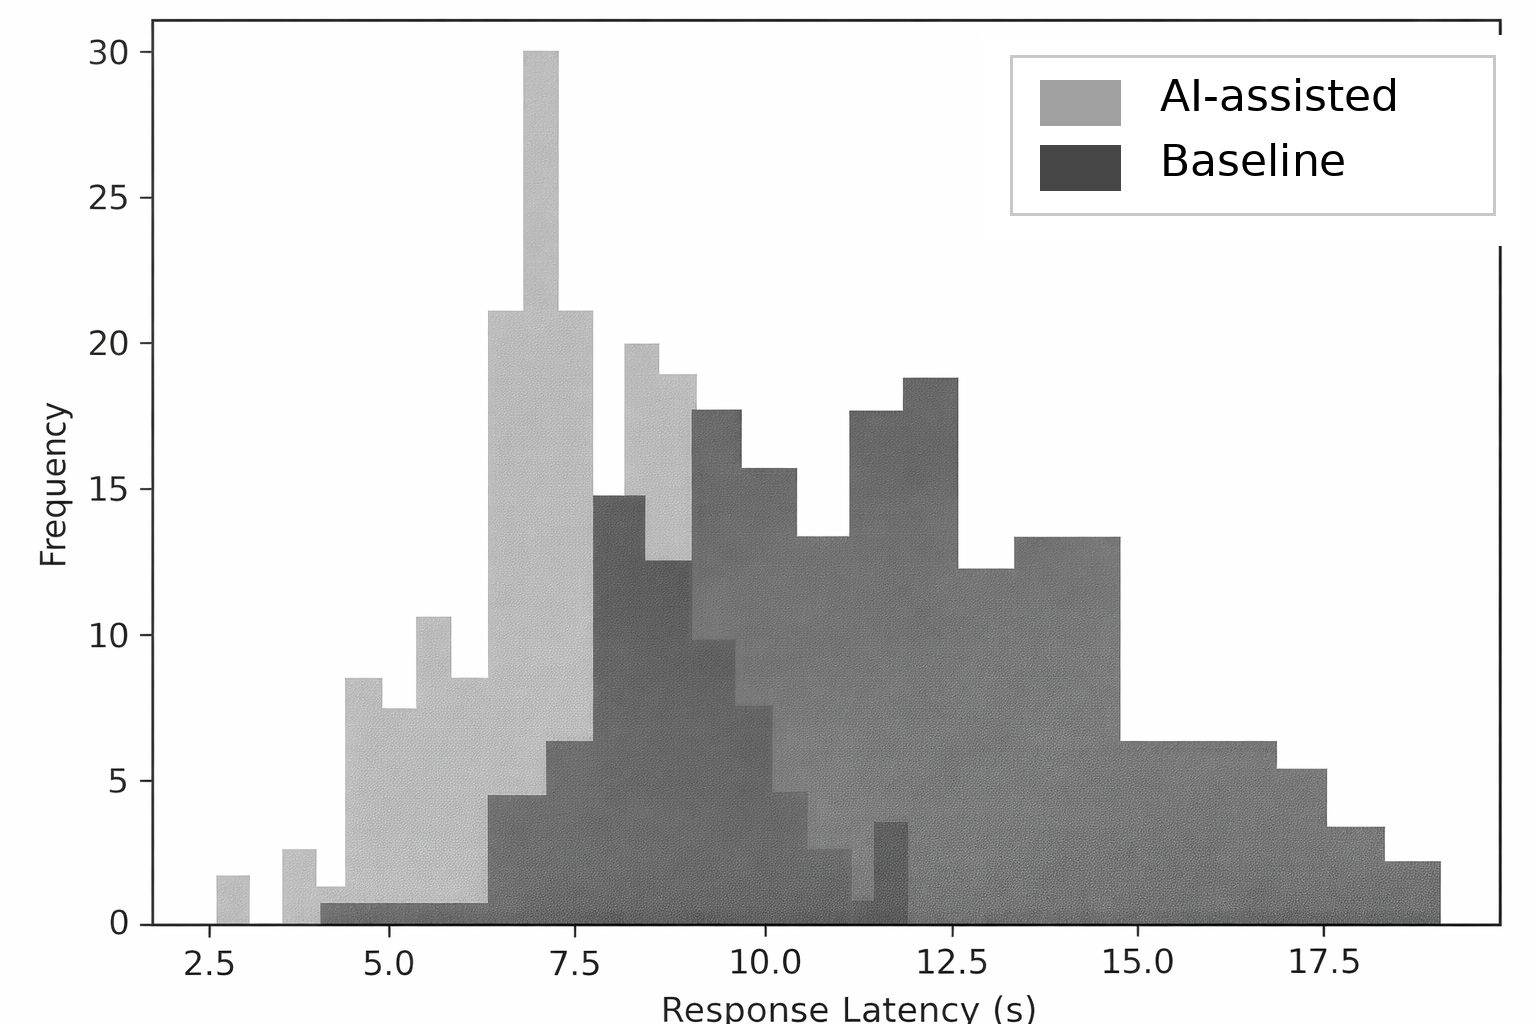
\includegraphics[width=0.9\linewidth]{fig_latency_distribution.png}
        \caption{Distribution of response latency under the baseline and AI-assisted conditions.}
        \label{fig:latency_distribution}
    \end{figure}

    \subsection{Workload, Trust, and Usability}
    Fig.~\ref{fig:workload_trust_summary} summarizes the subjective measures, and Table~\ref{tab:subscales} gives the subscale scores.
    The overall NASA--TLX score was 59.8 (SD 10.9) in the baseline condition and 46.2 (SD 9.6) in the AI-assisted condition, a difference of 13.6 points (paired test, $p < .05$; $d_{av} = 1.32$).
    The overall trust score was 3.4 (SD 0.6) in the baseline condition and 4.2 (SD 0.5) in the AI-assisted condition on the 5-point scale (paired test, $p < .05$; $d_{av} = 1.45$).
    The SUS score was 68.5 (SD 11.2) in the baseline condition and 81.7 (SD 9.4) in the AI-assisted condition ($d_{av} = 1.28$). No significance test was reported for the SUS.

    \begin{figure*}[t]
        \centering
        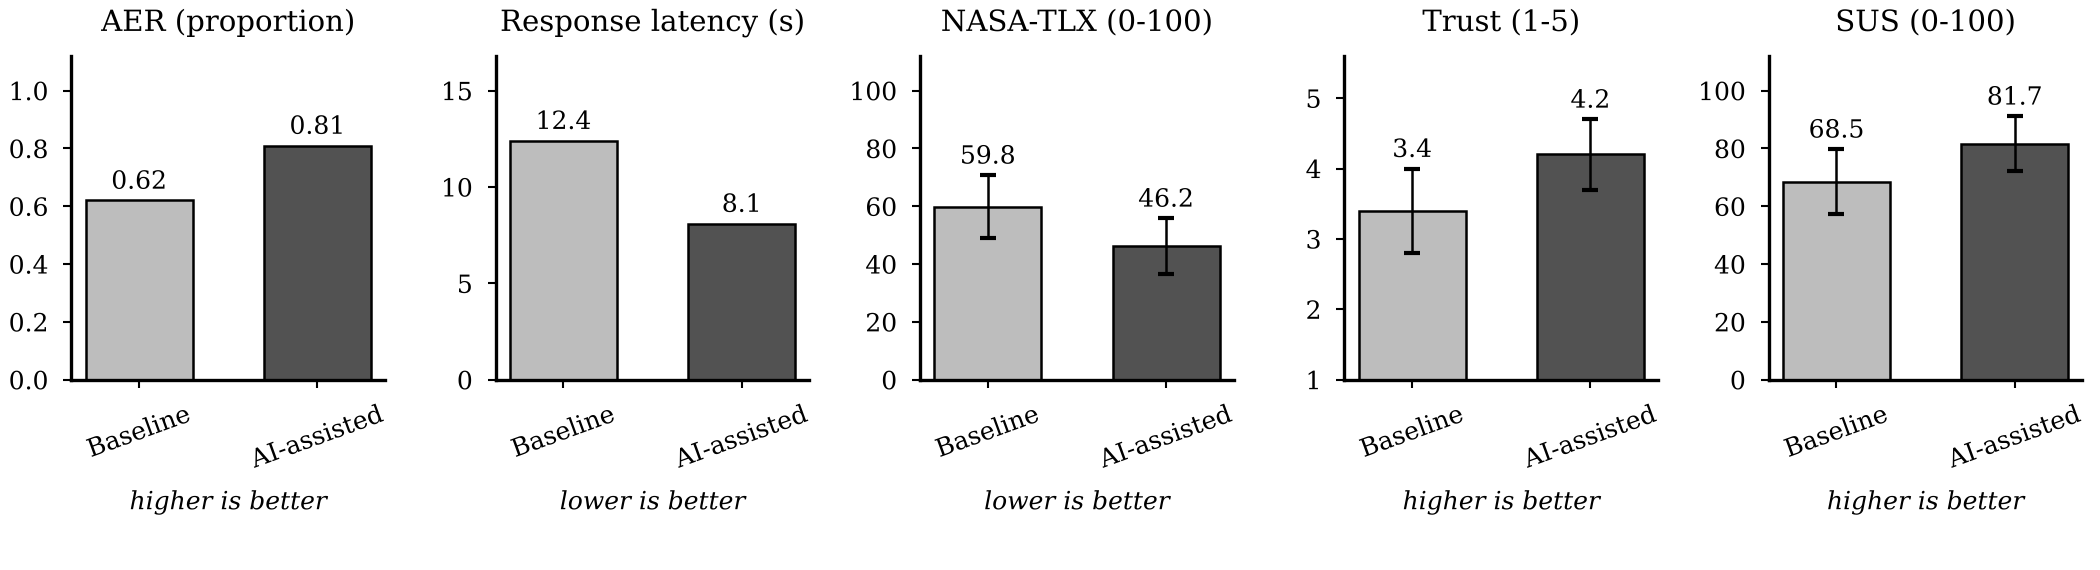
\includegraphics[width=0.95\linewidth]{fig_outcomes_summary.png}
        \caption{Primary and secondary outcomes in the baseline and AI-assisted conditions (values from Table~\ref{tab:primary}). Each outcome is shown on its own scale. Error bars show $\pm 1$ SD where SDs are available (not available for AER and response latency).}
        \label{fig:workload_trust_summary}
    \end{figure*}

    \begin{table}[t]
        \caption{Subscale Scores, M (SD)}
        \label{tab:subscales}
        \centering
        \begin{tabular}{lcc}
            \toprule
            \textbf{Subscale} & \textbf{Baseline} & \textbf{AI-assisted} \\
            \midrule
            \multicolumn{3}{l}{\emph{NASA--TLX (0--100)}} \\
            Mental demand & 63.4 (12.1) & 48.7 (10.5) \\
            Temporal demand & 58.9 (11.4) & 44.2 (9.8) \\
            Effort & 61.7 (13.0) & 49.1 (11.2) \\
            Frustration & 55.3 (14.6) & 41.8 (12.3) \\
            \midrule
            \multicolumn{3}{l}{\emph{Trust items (1--5)}} \\
            Perceived reliability & 3.2 (0.7) & 4.1 (0.6) \\
            Perceived predictability & 3.5 (0.8) & 4.2 (0.6) \\
            Perceived appropriateness & 3.4 (0.6) & 4.3 (0.5) \\
            \bottomrule
        \end{tabular}
    \end{table}

    \subsection{Escalated and Non-Escalated Trials (Descriptive)}
    \label{sec:res_escalation}
    Table~\ref{tab:escalation} reports, descriptively, the rates of appropriate deferral and inappropriate reliance in escalated and non-escalated trials of the AI-assisted condition. Appropriate deferral denotes deferring the decision for further confirmation when the situation warranted it. Inappropriate reliance denotes following the AI recommendation when this was not appropriate. These two sets of trials are not equivalent conditions. Escalation is triggered by high uncertainty or criticality, and it explicitly prompts human review. The differences in Table~\ref{tab:escalation} therefore cannot be attributed causally to escalation. The number of trials in each set was not available.

    \begin{table}[t]
        \caption{Behavior in Escalated vs.\ Non-Escalated Trials, AI-Assisted Condition (Descriptive)}
        \label{tab:escalation}
        \centering
        \begin{tabular}{lcc}
            \toprule
            \textbf{Metric} & \textbf{No escalation} & \textbf{Escalation triggered} \\
            \midrule
            Appropriate deferral rate & 0.21 & 0.47 \\
            Inappropriate reliance rate & 0.18 & 0.09 \\
            \bottomrule
        \end{tabular}
    \end{table}

    \subsection{Qualitative Observations}
    Table~\ref{tab:qualitative} summarizes recurring comments from the post-task interviews. These are informal observations. They were not systematically coded, and their prevalence was not recorded (Section~\ref{sec:measures}).

    \begin{table}[t]
        \caption{Informal Observations From Post-Task Interviews (Not Systematically Coded)}
        \label{tab:qualitative}
        \centering
        \begin{tabular}{p{0.30\linewidth}p{0.60\linewidth}}
            \toprule
            \textbf{Theme} & \textbf{Observation (paraphrased)} \\
            \midrule
            Reduced context switching & Recommendations reduced the need to cross-reference multiple sources. \\
            Usefulness of uncertainty cues & Participants used uncertainty cues to decide when to defer or seek confirmation. \\
            Accountability and control & The ability to override improved perceived safety and responsibility. \\
            \bottomrule
        \end{tabular}
    \end{table}

    %----------------------------------------\input{./080-discussion}
\section{Discussion}
\label{sec:discussion}
This section interprets the results from a human--machine systems perspective. In line with the JCS view \cite{Hollnagel2005JCS,Woods2006JCS}, we interpret the results at the level of the joint human--AI system. Because the AI-assisted condition differed from the baseline in several features at once, the interpretations below about \emph{which} features produced the effects are hypotheses, not demonstrated causal pathways.

\subsection{Action Execution in the Joint Human--AI System}
In the AI-assisted condition, the AER was higher and response latency shorter than with the dashboard. This is consistent with H1 and H2. Evaluating the system by action execution, rather than by prediction accuracy, follows directly from the JCS perspective. In AI decision-support research, however, evaluation is still dominated by accuracy and information quality \cite{Lai2023FAccT,Muller2022CHIWORK,Yang2022THMSReview}. Our results illustrate that what a human--AI system achieves depends on how support is structured to lead to action, not only on whether support is available.

Several features of the AI-assisted condition could explain the improvement: the presence of a recommendation, its action-oriented phrasing, the explicit uncertainty and criticality cues, and escalation. Our design does not separate these features. In particular, we cannot conclude that presenting recommendations in an action format, rather than a risk format, caused the improvement. A factorial design that varies the format while holding the other features constant is needed to test this (Section~\ref{sec:limitations}). Because the AER could not be decomposed, it also remains open whether the improvement came mainly from fewer wrong actions or from fewer late actions (Section~\ref{sec:lim_reporting}).

\subsection{Framework-Based Interpretation of the Results}
\label{sec:interpretation}
The following interpretation organizes the observed results along the ACHDF layers. It does not test the proposed mechanisms; it is a framework-based reading of the existing outcomes.
\emph{Action level:} the higher AER and lower latency (Table~\ref{tab:primary}) are consistent with the idea that uncertainty-aware adaptation of support helps operators move from risk interpretation to action.
\emph{Error-structure level:} in escalated trials, appropriate deferral was more frequent and inappropriate reliance less frequent than in non-escalated trials (Table~\ref{tab:escalation}). Because escalation is triggered by uncertainty and criticality and itself prompts human review, this pattern is descriptive. It is compatible with, but does not demonstrate, a protective effect of escalation against over-reliance.
\emph{Process level:} interview themes on reduced context switching (Table~\ref{tab:qualitative}) and lower NASA--TLX scores (Table~\ref{tab:subscales}) suggest that the AI-assisted condition changed the decision process.

\textbf{Workload as a possible explanation.} Lower workload is a plausible contributor to better action execution. The NASA--TLX, however, is a retrospective, subjective, condition-level measure, and we did not test whether the reduction in workload explains the improvement in AER (e.g., with a mediation analysis). This link should therefore be regarded as a possible explanatory mechanism, not a demonstrated pathway.

\subsection{Trust and Automation Bias}
Perceived trust was higher in the AI-assisted condition. Higher trust is not the same as \emph{calibrated} trust. Calibration requires that reliance matches the actual reliability of the advice \cite{Lee2004}. Showing calibration would require relating trust or reliance to the correctness of the AI's recommendations, trial by trial. The greater deferral in escalated trials is also not evidence of calibration, because escalation itself prompts human review. We therefore make no claim that ACHDF calibrates trust.

Similarly, automation bias can be directly assessed only on trials in which the AI's advice is wrong, by measuring how often participants accept it \cite{Parasuraman2010}. The study did not analyze behavior on trials with erroneous AI recommendations, so it cannot show whether ACHDF reduces automation bias. This is an important topic for future work.

\subsection{Ecological Validity of Escalation}
In the study, participants could defer a decision when the system escalated. In real time-critical emergencies, deferral may not be feasible or may itself be costly: an operator may have to act on uncertain information before an evacuation window closes. The lower inappropriate reliance observed in escalated trials may therefore not carry over to settings where deferral is constrained, and forced action under uncertainty might change both reliance and workload. Future studies should assign explicit costs to deferral and include forced-choice conditions.

    \begin{table}[t]
        \caption{Observed Findings and Candidate Design Implications (to Be Tested Component-Wise)}
        \label{tab:design_implications}
        \centering
        \begin{tabular}{p{0.38\linewidth} p{0.52\linewidth}}
            \toprule
            Observed finding & Candidate design implication \\
            \midrule
            Higher AER, lower latency & Action-oriented recommendations \\
            Lower NASA--TLX & Consolidated information structuring \\
            Higher perceived trust & Explicit uncertainty and criticality cues \\
            \bottomrule
        \end{tabular}
    \end{table}

\subsection{Design Implications}
Within the scope of the evaluated task, the results suggest that human--AI decision support systems may benefit from (1) representing uncertainty explicitly, (2) providing action guidance rather than only passive information display, and (3) adapting the level and form of support to uncertainty and criticality through human-in-the-loop escalation, while leaving final authority with the human \cite{Assaad2023TAS,Zhang2022THMS,Bach2024Access,Parasuraman2000LOA}. Table~\ref{tab:design_implications} lists these candidate implications. Because the components were not manipulated separately, each implication should be tested individually. Whether they transfer to other safety-critical domains, such as healthcare, transportation, and industrial safety \cite{PerezCerrolaza2024CSUR,Farhan2025TCE}, has not been tested here (Table~\ref{tab:achdf_transferability}).

    %---------------------------------\input{./090-futurework}
    \section{Limitations and Future Work}
    \label{sec:limitations}

    \subsection{Bundled Intervention}
    The AI-assisted condition differed from the baseline in several features at once. The study therefore estimates the effect of the integrated ACHDF configuration and cannot attribute effects to individual components (uncertainty display, action format, escalation, guardrails). Future work should use factorial or ablation designs.

    \subsection{Trust Calibration and Automation Bias}
    Trust was measured as a self-reported attitude at the condition level, and behavior on trials with erroneous AI recommendations was not analyzed. Hence, neither calibration nor automation bias could be assessed directly. Future studies should include trials with incorrect advice and measure reliance trial by trial.

    \subsection{Domain and Population Generalizability}
    The evaluation was conducted only with disaster-response scenarios in a simulated setting. Participants were not required to have domain expertise, and the sample was not composed specifically of emergency-management professionals. Trained emergency operators may behave differently: they may rely less on recommendations, use different heuristics, or experience different workload. Generalization to other domains (e.g., medical triage, autonomous driving supervision, traffic management) and to professional operators remains future work. The ecological limits of deferral (Section~\ref{sec:discussion}) also belong here.

    \subsection{Reporting and Analysis Limitations}
    \label{sec:lim_reporting}
    Several analyses and details requested for a complete account of the study could not be provided, because the trial-level data and some study materials were not available for re-analysis. The affected results should be interpreted with corresponding caution:
    \begin{itemize}
        \item \emph{Inferential statistics.} Only the significance thresholds of the original paired tests are available. Exact test statistics, 95\% confidence intervals, assumption diagnostics, the paired effect size $d_z$, order-effect analyses, and multiplicity-corrected $p$-values could not be computed. SDs for the AER and response latency are not available, and the paired test used for each outcome is not documented. No a priori power analysis was reported; the sensitivity analysis (Section~\ref{sec:participants}) indicates adequate power only for effects of about $d_z \geq 0.40$.
        \item \emph{AER construction.} The procedure for defining the appropriate action and the length of the time window are not documented in detail, and the AER could not be decomposed into action correctness and timeliness. Consequently, it cannot be determined whether execution failures were due to wrong actions or to delays.
        \item \emph{Task and materials.} The number and composition of scenarios (by uncertainty and criticality), the full set of response options, the per-trial time limit, the matching of scenario difficulty, the training content and any pass criterion, and interface screenshots are not reported. This limits reproducibility.
        \item \emph{System implementation.} The risk model's estimation and calibration procedure, the criticality scale and thresholds, and the specific guardrail rules are not reported. The evaluation therefore concerns the interaction design as experienced by participants, not the validity of these components.
        \item \emph{Measures.} The trust items have no published validation and their internal consistency could not be estimated. The interview data were not systematically coded. The number of escalated trials is not available.
    \end{itemize}
    Future studies should preregister their analyses and share trial-level data and materials so that these analyses can be reported in full.

    \subsection{Long-Term Trust Effects}
    The study captured only short-term effects within a single session. Trust and reliance may change with longer exposure to the system and to its escalation behavior, which calls for longitudinal field studies.

    %-------------------------------\input{./092-conclusion}
\section{Conclusion}
This paper presented ACHDF, an action-centered human--AI decision framework that instantiates the joint cognitive systems perspective for disaster-response decision support. ACHDF combines uncertainty-aware risk estimation, guardrailed recommendations, and uncertainty- and criticality-triggered escalation, while the human keeps final decision authority. In a within-subjects study with 52 participants, the integrated ACHDF configuration, compared with a conventional dashboard, was associated with a higher action execution rate, shorter response latency, lower self-reported workload, and higher perceived trust and usability. The study did not isolate individual components, assess trust calibration or automation bias directly, or test other domains or professional operators. These questions define the next steps toward validated design principles for human--AI decision support under uncertainty.

\section*{Acknowledgment}
The author thanks the study participants for their time and insights, and colleagues in human--machine systems and human-centered AI research for valuable discussions.




%% How to support DOI (Digital Obect Identifier) in reference section:
% \url{https://ctan.org/tex-archive/macros/latex/contrib/IEEEtran/bibtex?lang=en}
% \url{https://people.kth.se/~maguire/myIEEEtran.bst}
% \url{https://ipfs-sec.stackexchange.cloudflare-ipfs.com/tex/A/question/67444.html}
% \url{https://ipfs-sec.stackexchange.cloudflare-ipfs.com/tex/A/question/394811.html}
\bibliographystyle{IEEEtranDOI}

%% Type1: sorting, keep sequence of reference numbers that user typed.
%\bibliographystyle{IEEEtranDOI} 

%% Type2: sorting, re-arrange sequence of reference numbers that user typed
% for ascending cite number.
% \bibliographystyle{IEEEtranDOI}

%% Add reference papers
\bibliography{reference-data}



% omitting for THMS journal
% 


% === Author Biographies ===
\vspace{2em} % (필요 시 조절)
\noindent
\begin{minipage}{\linewidth}
\begin{IEEEbiography}[{
\includegraphics[width=1in,height=1.25in,clip,keepaspectratio]{./fig_author-lim2.png}}]{Geunsik Lim}
received the B.S. degree in Computer Science and Engineering from Ajou University, South Korea, in 2003, and the M.S. and Ph.D. degrees in Electrical and Computer Engineering from Sungkyunkwan University, South Korea, in 2014 and 2023, respectively. He is currently a principal software engineer at Samsung Electronics in South Korea. His research interests include system optimization, operating systems, software platforms, and on-device artificial intelligence. 
\end{IEEEbiography}
\end{minipage}


\end{document}
